\documentclass{beamer}

\usepackage[british]{babel}
\usepackage{graphicx,hyperref,ru,url}
\usepackage{amsmath}
\usepackage{qrcode}
\usepackage{hyperref}

% The title of the presentation:
%  - first a short version which is visible at the bottom of each slide;
%  - second the full title shown on the title slide;
\title[State of the lab - 2019]{Artificial Neural networks for the prediction of phage protein function }

% Optional: a subtitle to be dispalyed on the title slide
%\subtitle{Show where you're from}

% The author(s) of the presentation:
%  - again first a short version to be displayed at the bottom;
%  - next the full list of authors, which may include contact information;
\author[A. Cantu]{Adrian Cantu}

% The institute:
%  - to start the name of the university as displayed on the top of each slide
%    this can be adjusted such that you can also create a Dutch version
%  - next the institute information as displayed on the title slide
\institute[]{
  San Diego State University \\
  Computational Science Research Center}

% Add a date and possibly the name of the event to the slides
%  - again first a short version to be shown at the bottom of each slide
%  - second the full date and event name for the title slide
\date[05/21/2019]{
  May 21th 2019}

\begin{document}

\begin{frame}
  \titlepage
  \centering
\end{frame}


\begin{frame}{BacterioPhage}
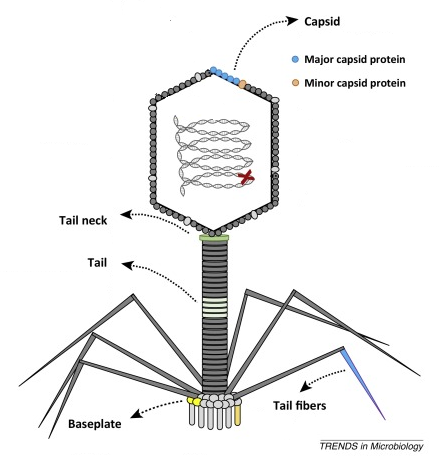
\includegraphics[width=0.70\textwidth]{img01}
\end{frame}

\begin{frame}{Databases}
\begin{table}[!htb]
\begin{tabular}{llll}
\hline
Class                                                       & Raw sequences & \begin{tabular}[c]{@{}l@{}}After manual\\ curation\end{tabular} & \begin{tabular}[c]{@{}l@{}}After 90\%\\ dereplication\end{tabular} \\ \hline
Major capsid                                                & 112,987       & 105,653                                                         & 13,172                                                             \\ \hline
Minor capsid                                                & 2,901         & 1,903                                                           & 656                                                                \\ \hline
Baseplate                                                   & 75,599        & 19,293                                                          & 2,090                                                              \\ \hline
Major tail                                                  & 66,513        & 35,030                                                          & 3,249                                                              \\ \hline
Minor tail                                                  & 94,628        & 80,467                                                          & 3,886                                                              \\ \hline
Portal                                                      & 210,064       & 189,143                                                         & 18,622                                                             \\ \hline
Tail fiber                                                  & 29,132        & 18,514                                                          & 3,191                                                              \\ \hline
Tail shaft                                                  & 37,885        & 35,570                                                          & 4,933                                                              \\ \hline
Collar                                                      & 4,224         & 3,709                                                           & 1,262                                                              \\ \hline
\begin{tabular}[c]{@{}l@{}}Head-Tail\\ joining\end{tabular} & 60,270        & 58,658                                                          & 6,713                                                              \\ \hline
Other                                                  & 733,006        & -                                                          &  162,709                                                             \\ \hline
\end{tabular}
\caption{The classes database by the numbers}
\label{tab:my-table}
\end{table}
\end{frame}

\begin{frame}{Protein Sequences}
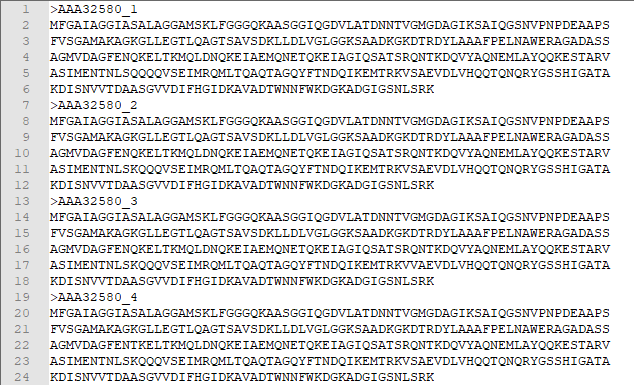
\includegraphics[width=0.90\textwidth]{fasta}
\end{frame}

\begin{frame}{F:Sequence --$>$ Function}
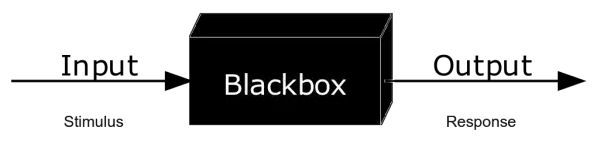
\includegraphics[width=0.90\textwidth]{blackbox}
\end{frame}

\begin{frame}{Artificial Neural Networks}
\begin{minipage}[t]{0.5\textwidth}
  \centering\raisebox{\dimexpr \baselineskip-\height}{%
  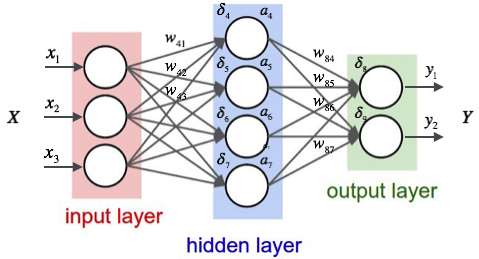
\includegraphics[width=0.90\textwidth]{img03_ANN}}
\end{minipage}\hfill
\begin{minipage}[t]{0.5\textwidth}
ANN have been shown to be universal approximators of \underline{continuous} functions in $\mathbb{R}^n$ \\
$$
d=\left(\int_0^{2\pi}|f_1(t)-f_2(t)|^p dt\right)^\frac{1}{p}
$$
where $1<p<\infty$
\end{minipage}
\end{frame}


\begin{frame}{Artificial Neural Networks}
\begin{minipage}[t]{0.5\textwidth}
$$
\begin{pmatrix}
Z_1\\ 
Z_2\\ 
\vdots \\ 
\vdots\\ 
\vdots\\ 
\vdots\\ 
\vdots\\ 
Z_{408}\\ 
\end{pmatrix}
\begin{matrix}
\\ 
\\ 
\\ 
\\ 
=X\\ 
\\ 
\\ 
\\ 
\\
\end{matrix}
$$
\end{minipage}\hfill
\begin{minipage}[t]{0.5\textwidth}
$$
\begin{pmatrix}
Y_1\\ 
Y_2\\ 
Y_3\\ 
Y_4\\ 
Y_5\\ 
Y_6\\ 
Y_7\\ 
Y_8\\ 
Y_{9}\\ 
Y_{10}\\
Y_{11}
\end{pmatrix}
\begin{matrix}
\\ 
\\ 
\\ 
\\ 
\\ 
=Y\\ 
\\ 
\\ 
\\ 
\\ 
\\ 
\end{matrix}
$$
where $\sum_{n=1}^{11}Y_n=1$
\end{minipage}
\end{frame}

\begin{frame}{The 'black box' function}
\scalebox{0.7}{%
$Y=F(X)=\underbrace{[10*200]}_{W_3}\left(\underbrace{[200*200]}_{W_2}\left(\underbrace{[200*408]}_{W_1}\underbrace{[408*1]}_X+\underbrace{[200*1]}_{\delta_1}\right)+\underbrace{[200*10]}_{\delta_2}\right)+\underbrace{[10*1]}_{\delta_1}
$} \\
\begin{center}
289,866 Trainable parameters
\end{center}
\end{frame}

\begin{frame}{Precision and Recall}
\begin{minipage}[t]{0.3\textwidth}
\vspace{-2cm}
$$precision = \frac{TP}{TP+FP}$$
\end{minipage}
\begin{minipage}[t]{0.3\textwidth}
$$recall= \frac{TP}{FN+TP}$$
\end{minipage}
\begin{minipage}[t]{0.3\textwidth}
\vspace{2cm}
$$F1 = \frac{2 \cdot precision\cdot recall}{precision+ recall}$$
\end{minipage}
\hfill
\end{frame}

\begin{frame}{Accuracy}
$$
\begin{matrix}
 & Precision & Recall & f1-score & Support\\ 
Major\ capsid & 0.88 & 0.92 & 0.90 & 1232\\ 
Minor\ capsid & 0.27 & 0.57 & 0.36 & 51\\ 
Baseplate & 0.54 & 0.87 & 0.67 & 180\\ 
Major\ tail & 0.82 & 0.88 & 0.85 & 289\\ 
Minor\ Tail & 0.65 & 0.77 & 0.70 & 345\\ 
Portal & 0.87 & 0.90 & 0.88 & 1640\\ 
Tail\ Fiber & 0.54 & 0.67 & 0.60 & 272\\  
Tail\ shaft & 0.91 & 0.94 & 0.93 & 444\\ 
Collar & 0.75 & 0.80 & 0.77 & 129\\ 
Head-Tail\ Joining & 0.74 & 0.84 & 0.79 & 647\\
Other & 0.97 & 0.93 & 0.95 & 15254\\ 
 &  &  &  & \\ 
weighted\ avg & 0.82 & 0.79 & 0.79 & 675 
\end{matrix}
$$
\end{frame}



\begin{frame}{Results Confusion matrix}
\scalebox{0.95}{%
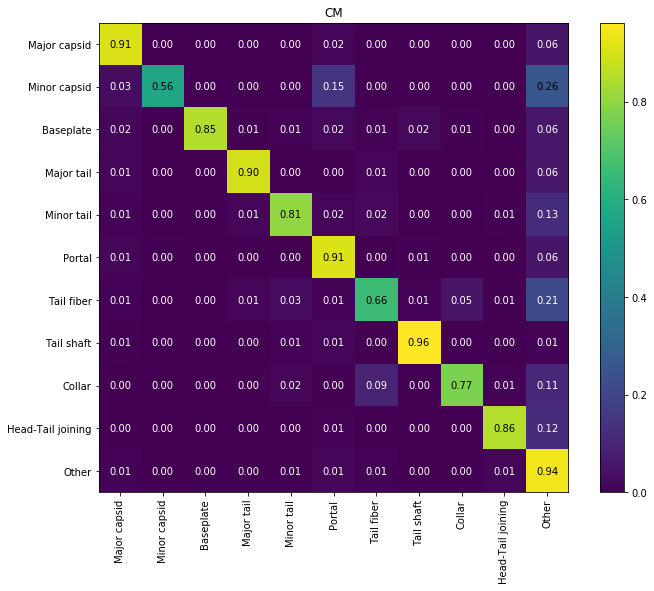
\includegraphics[width=0.90\textwidth]{cm_recall}
}
\end{frame}

\begin{frame}{Weighted average}
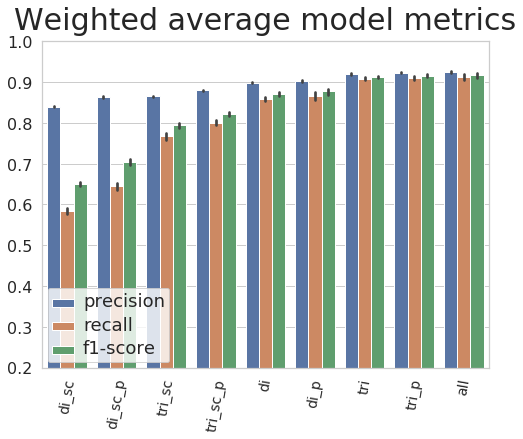
\includegraphics[width=0.90\textwidth]{avg_score_master}
\end{frame}


\begin{frame}
\begin{table}[]
\caption{Side chain grouping}
\begin{tabular}{|l|l|}
\hline
Hydrophobic     & A,I,L,M,V \\ \hline
Hydrophylic     & N,Q,S,T   \\ \hline
Small turn      & G,P       \\ \hline
disulfide       & C         \\ \hline
Positive charge & H,K,R     \\ \hline
Negative charge & D,E       \\ \hline
Aromatic        & F,W,Y     \\ \hline
\end{tabular}
\end{table}
\end{frame}



\begin{frame}{Per class f1-score}
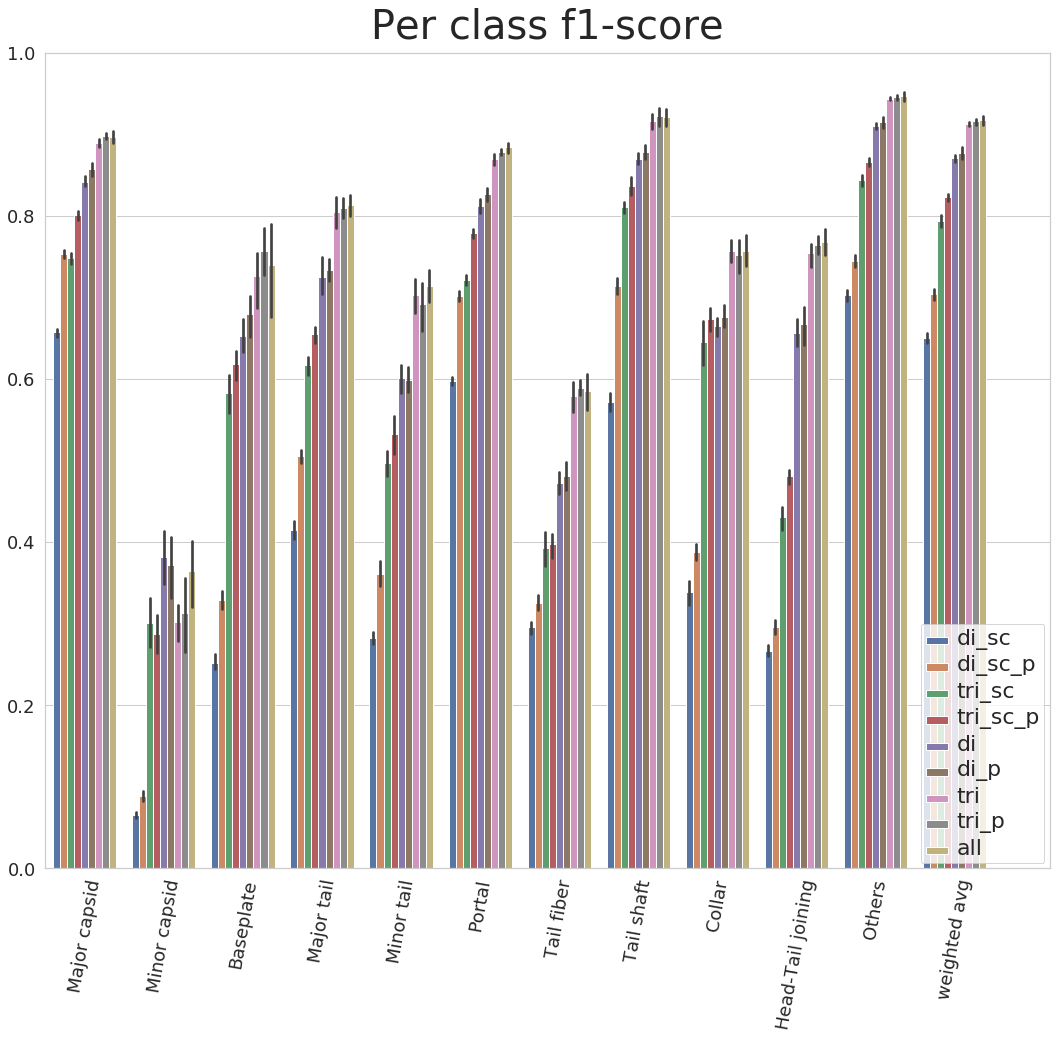
\includegraphics[width=0.75\textwidth]{f1_score_master_per_class}
\end{frame}

\begin{frame}{Per class f1-score}
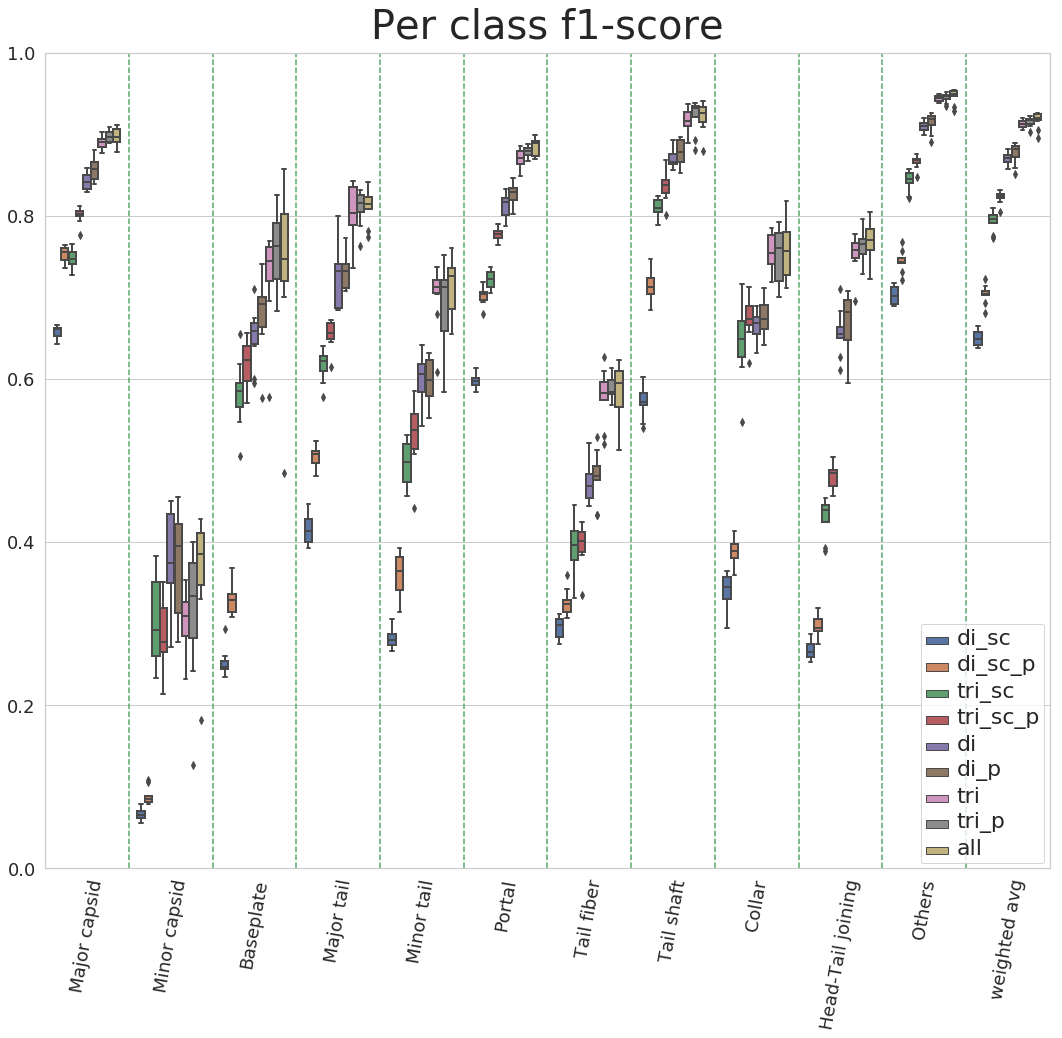
\includegraphics[width=0.75\textwidth]{f1_score_master_per_class_boxplot}
\end{frame}

\begin{frame}{website}
\begin{center}
\qrcode{http://edwards.sdsu.edu/PhANNies/}
\url{http://edwards.sdsu.edu/PhANNies/}
\end{center}
\end{frame}

%\begin{frame}{Conclusions}
%\begin{itemize}
%\item [-] ANN is slow to train but fast to run.
%\item [-] Robots will rule the world
%\end{itemize}
%\end{frame}

\end{document}
